\documentclass[a4paper,12pt]{extarticle}
\usepackage[utf8]{inputenc}
\usepackage[german]{babel}
\usepackage{amsmath}
\usepackage{amsthm}
\usepackage{amsfonts}
\usepackage{amssymb}
\usepackage{graphicx}
\usepackage{units}
\usepackage{wrapfig}
\usepackage{float}
\usepackage{tikz}
\usepackage{tkz-euclide}
\usetkzobj{all}
\usetikzlibrary{arrows.meta}
\usepackage{multicol}
\usepackage{caption}
\usepackage{verbatim}
\usepackage{hyperref}
\usepackage[european]{circuitikz}
\usepackage{adjustbox}
\usetikzlibrary{shapes.geometric}

\newenvironment{Figure}
  {\par\medskip\noindent\minipage{\linewidth}}
  {\endminipage\par\medskip}


\usepackage[left=2.5cm,right=2.5cm,top=1.8cm,bottom=2cm]{geometry}

\usepackage{pgfplots}
\usepackage{titlesec}

\titleformat*{\section}{\Large \bfseries \sffamily}
\titleformat*{\subsection}{\large \sffamily}


%\date{Abgabe am 12.09.2016}


\newtheoremstyle{problemstyle}  % <name>
        {3pt}                                               % <space above>
        {3pt}                                               % <space below>
        {\normalfont}                               % <body font>
        {}                                                  % <indent amount}
        {\sffamily \bfseries}                 % <theorem head font>
        {\normalfont\bfseries\\}         % <punctuation after theorem head>
        {.5em}                                          % <space after theorem head>
        {}                                                  % <theorem head spec (can be left empty, meaning `normal')>
\theoremstyle{problemstyle}

\newtheorem{problem}{Aufgabe}




\begin{document}

\pagenumbering{gobble}

\begin{multicols}{2}
\parbox{2.5cm}{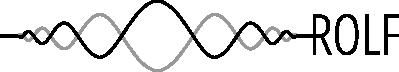
\includegraphics[width=2.5cm]{../task/images/logo_scaled.pdf}}
\parbox{4.5cm}{\centering{\Large \textsf{Notizen zum Seminar Mechanik}\\{\small Maximilian Marienhagen\\\url{pankratius.github.io/rolf}}}}
\section*{Einfache Bewegungen}
\begin{itemize}
\item Messung von Strecken $s$ und Wahl eines Ursprungspunkts, Def. von $v$ und $a$ durch Anstiege
\item Fläche unter $v-t-$Diagramm ist $s$
\begin{itemize}
\item $v$ konst. $\implies s=vt$
\item $a$ konst. $\implies s=\frac{1}{2}at^2$
\end{itemize}
\item kompliziertere eindimensionale Bewegungen als Superposition
\end{itemize}
\section*{Newtonsche Axiome}
\begin{align}
\vec{F} &= m \vec{a} & \vec{F}_{AB} &=-\vec{F}_{BA}
\end{align}
Vektorcharakter beachten!
\section*{Häufige Kräfte}
\begin{itemize}
\item Gewichtskraft in Erdnähe $F=mg$
\item Reibung $F\leq \mu F_N$(Richtung beachten)
\end{itemize}
\begin{problem}
Auf einer horizontalen Ebene liegt ein Körper der Masse $M$, wobei der Reibungskoeffizient zwischen Körper und Ebene $\mu$ ist. Mit dem Körper ist ein frei in der Höhe $h$ hängender Körper der Masse $m$ durch eine inelastische Schnur über eine Umlenkrolle verbunden. Nach welcher Zeit landet kommt dieser am Boden an?  
\end{problem}
\section*{Energierhaltung}
$\sum E = konst.$ mit kinetischer Energie und Bewegungsenergien ($\frac{1}{2}Dx^2$, $mgh$...)\\
\begin{problem}Finde $v,x,h...$ bei schiefer Ebene, Federschwinger etc. wenn jeweils anderes gegeben ist
\end{problem}
\section*{Impulserhaltung}
$\sum \vec{p} = konst.$ mit $\vec{p}=m\vec{v}$
\begin{problem}
Auf reibungsfreien Gleisen fährt ein Waggon der Masse $10t$ mit einer Geschwindigkeit von $3\frac{m}{s}$ auf einen ruhenden Waggon der Masse $20t$ zu. Beide kuppeln sich automatisch zusammen und rollen gemeinsam weiter. Wie groß ist die Geschwindigkeit des Zugs?
\end{problem}
\section*{Fortsetzungsmöglichkeiten}
\begin{itemize}
\item Stöße (elastisch, inelastisch, teilelastisch)
\item Gravitation (Kraft, Energie...)
\item Würfe (Superpositionsprinzip, Wurfweite...)
\item Rotation
\item Begriff der Arbeit im Kontext der Energieerhaltung

\end{itemize}
\end{multicols}
\end{document}